
\chapter{外文资料的书面翻译}

外文资料部分翻译了与本论文主题相关的两篇论文,其研究重点在于通过线圈或电流激发出扰动场从而达到对 ELM 的弱化和抑制效果。


\begin{translationbib}
  \item Sun Youwen, Liang Yunfeng, Liu Yueqiang and \textit{et al}. Nonlinear Transition from Mitigation to Suppression of the Edge Localized Mode with Resonant Magnetic Perturbations in the \east Tokamak. Physical review letters (2016). 117. 115001. 10.1103/PhysRevLett.117.115001. 
  \item Liang Yunfeng, Gong X. Z. , Gan K. F. and \textit{et al}. Magnetic Topology Changes Induced by Lower HybridWaves and their Profound Effect on Edge-Localized Modes in the \east Tokamak. Physical Review Letters (2013). 110. 235002. 10.1103/PhysRevLett.110.235002. 
\end{translationbib}


\title{\textbf{ \east  托卡马克上低杂波引起的磁拓扑变化及其对 ELM 的显著影响\\Magnetic Topology Changes Induced by Lower Hybrid Waves and their Profound Effect on Edge-Localized Modes in the \east Tokamak} [1]}

{\heiti 摘要:} {\kaishu 当低杂波和离子回旋共振加热作用在 \Hmode 的等离子体,在  \east  上观测到了强烈的减弱 ELM 的作用。这种效果是由于低杂波引起的螺旋电流丝沿着磁力线在刮削层中不断流动的效果。和共振磁扰动的效果类似,在低杂波运作期间也出现了束流在偏滤器上打击点分裂的现象。通过在磁力线追踪程序中加入螺旋电流丝,本文也定性地模拟了其对磁拓扑结构的改变的作用。}

% TODO Add figure 


对聚变能源研究及相关技术的巨大挑战来自于如何将炽热的等离子体约束住,使得接触等离子体的材料在运行期间维持一个可以接受(稳态和瞬态)的热负荷及粒子束流强度。
当托卡马克中的等离子体工作在高约束(\Hmode)状态的时候,等离子体能量约束时间显著增长。然而其后果则是等离子体边界上压强有着更大的梯度,连带着还有边界上增强了的电流密度,它可以超过驱动磁流体不稳定性的阈值,这被称为 ELM。 ELM 会导致拟周期性的大量能流和粒子流损失,因而也会导致对接触的等离子体材料的严重损害,下一代的聚变设备,如 \iter 和 DEMO 装置,需要一种可靠的手段来控制或者抑制剧烈的边界区域模。

共振磁扰动(RMP)改变了等离子体的磁拓扑结构,已经被用在 \ddd 装置内完全抑制 ELM ; JET, \mast 和 AUG 的实验中,则起到了削弱 ELM 的作用,增加 ELM 的频率的同时大大降低每一次 ELM 发生的幅度,MAST 和 ORG 装置上面得到实验。尽管其物理机制还不是很清楚,但从这些装置上得到的实验结果都表明是磁拓扑起到很关键的作用,深刻地影响了边界磁流体稳定性以及等离子体-壁(特别是对于偏滤器)相互作用。


目前来说,在所有现存的以共振磁扰动减弱或抑制 ELM 的实验中,磁扰动均由腔内或者腔外的线圈系统所激发。腔内的磁扰动线圈已在 \iter 设计上被考虑并做出了设计,用于抑制 ELM 的发生。但在未来的聚变反应堆中(如 DEMO),腔内的磁扰动线圈可能不现实。于是其他可以改变磁拓扑以控制 ELM 机制,对于下一代的托克马克是很有吸引力的。

近期 \east 上面的研究结果表明,低杂波和共振磁扰动的效果类似,也可以改变磁拓扑以作为一种有效的减弱或抑制 ELM 的手段。这篇快报阐述了低杂波对 ELM 表现的影响及偏滤器平板上的热负荷分布;同时记录了低杂波驱动下产生的,在刮削层中沿着磁力线流动的螺旋电流丝的实验结果(该螺旋电流丝并不随时间旋转)。实验观测到的由螺旋电流丝引起的三维边界磁拓扑改变和磁力线追踪程序所做的估计之间进行了对比。

% FIXME 翻译不会翻
\east (大半径和小半径分别是 \SI{1.85}{\metre} 和 \SI{0.45}{\metre}) 是为了实现稳定的长脉冲、高参数的 \Hmode 等离子体而建造的装置,它的位型与加热设备均与 ITER 类似,即有着灵活可调的 double null, lower single null (SN) 或 upper (SN) 极向偏滤器位型并主要是射频加热。\east 中的低杂波系统工作在 \SI{2.45}{\giga\hertz},一个阵列由 20 个波导天线组成,四列五行,安装在低场侧中间,最大输出功率是 \SI{2}{\mega\watt}。低杂波最初被设计用于芯部等离子体电流驱动,通过电子朗道阻尼将动量转移给等离子体,峰值平行方向波折射率约 2.1。并且可以在没有离子回旋共振加热的条件下仍实现长脉冲下的\Hmode 。然而和其他设备上的实验类似,在等离子体边界上面损失了相当显著的低杂波功率,特别是当等离子体密度较高时,这是由快波和粒子之间复杂的耦合问题所导致的。

通过在离子回旋共振加热占主导的\Hmode 等离子体中调制低杂波功率,团队研究了低杂波对于 ELM 的特性影响,如图 1。这项实验在一次腔壁涂锂之后不久进行,通过输入功率是 \SI{1}{\mega\watt} 的粒子回旋共振加热驱动,目标 \Hmode 等离子体有着下 SN 位型且运行在一个相对高密度的工作区。在边界上的安全因子是 $q_{95}=3.8$,环向等离子体电流为 $I_p=\SI{500}{\kilo\ampere}$ 且环向场 $B_t=\SI{1.8}{\tesla}$,底部的三角形变系数是 $\delta_L=0.45$。在中心处线平均的电子密度 $<n_e> $ 约 $\SI{4.7e19}{\meter^{-3}}$,Greenwald 分数约 0.9,以及 H 系数(H98y)在 \Hmode 阶段约 0.8。

\begin{figure}[h]
  \centering
  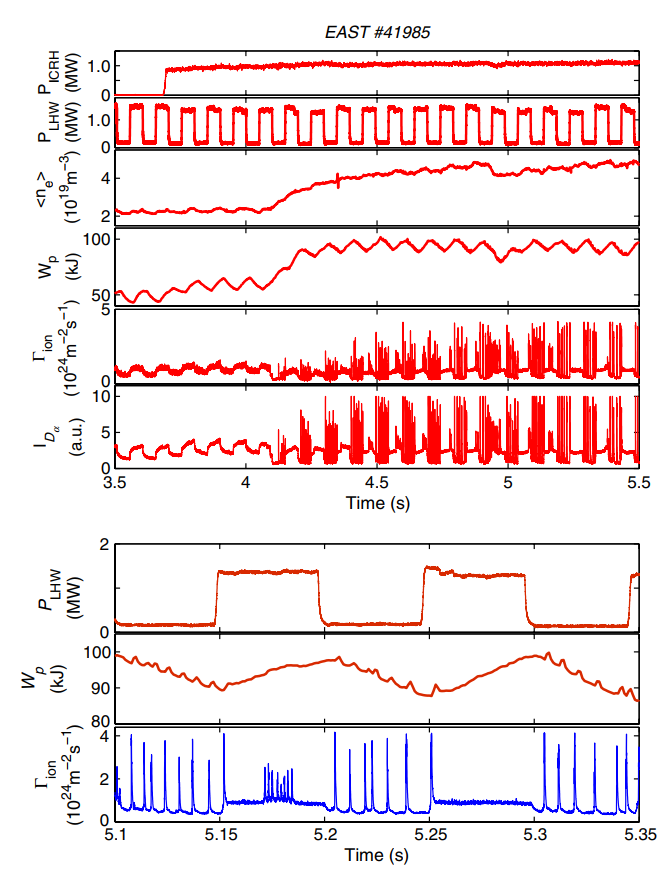
\includegraphics[width=0.85\columnwidth,keepaspectratio]{translate/liang_1.png}
  \caption*{图~1\hskip1em 低杂波功率调制对 ELMs 的影响。从上到下的时间序列分析分别为 ICRH 和 LHW 的注入功率,中心线平均密度,等离子体能量,峰值粒子流强和 外侧偏滤器平板上 $D_\alpha$ 的射线强度。在底部将低杂波功率、等离子体储能和偏滤器上峰值粒子流强的一小段时间区间放大观察。}
  \label{fig:liang_figure1}
\end{figure}

这套低杂波系统功率设置在 \SI{1.3}{\mega\watt},调制频率为 \SI{10}{\hertz},单个周期内运转时长占比 50\%,即一个周期内低杂波关闭的时间是\SI{50}{\milli\second},这个时间大概是能量约束时间的一半。如果没有低杂波加热的话,ELM 的频率是相当规律的,大概在 \SI{150}{\hertz};当低杂波系统打开之后,ELM 消失了或者偶尔地以更高频($\sim\SI{600}{\hertz}$)出现,如图 1 下侧,此时观察到落到偏滤器平板上的 ELM 的脉冲粒子流强显著地减小为原来的 $1/2$,而 ELM 间隙时的粒子数则约增强为原来的 $2$ 倍,但仍然低于运行在 \Lmode 时。一旦到达\Hmode 工作区,等离子体所具有的能量 $W_p$ 约增长为原来的 2 倍,从 $\sim 50$ 到 $\sim\SI{100}{\kilo\joule}$;在此后的低杂波功率调制期间,它的变化幅度比较微弱($\pm 5\%$区间)。低杂波系统停止工作的瞬间偏滤器平板接收到的离子流强会迅速减小,这可能说明低杂波功率不仅被芯部吸收,也部分沉积在了刮削层中。

% FIXME translation
\east 实验中,不管工作在\Lmode 还是\Hmode ,低杂波运行时刮削层中都观测到了 5 条螺旋辐射带(Helical radiation belt, HRB)。螺旋辐射带的数量和低杂波天线阵列的行数相等。\east 使用氦气放电使其结构更清楚而不影响其特征,图 2 展示了两个切向方向上可见光波段的照片作为例子,这是 \east 环形腔两侧氦气等离子体放电过程中低杂波施加时所出现的现象。
目标等离子体($\SI{300}{\kilo\ampere}$,$B=\SI{2}{\tesla}$, $q_{95}=\approx 8$) 由 \SI{0.7}{\mega\watt} 的低杂波加热,是 double null 的位型。在赤道面,等离子体分界面到外侧限制器的间隔大概在 \SI{8}{\centi\metre}。螺旋辐射带出现在低场侧,经过低杂波天线前方,同时在刮削层中沿着磁场线向上、下沿偏滤器流动。在低杂波天线前方,原等离子体边界 \SI{1}{\centi\meter} 之外的地方作为地点模拟得到的磁力线,在位置和螺旋角上都较好地吻合了实验观测到的螺旋辐射带。


\begin{figure}[h]
  \centering
  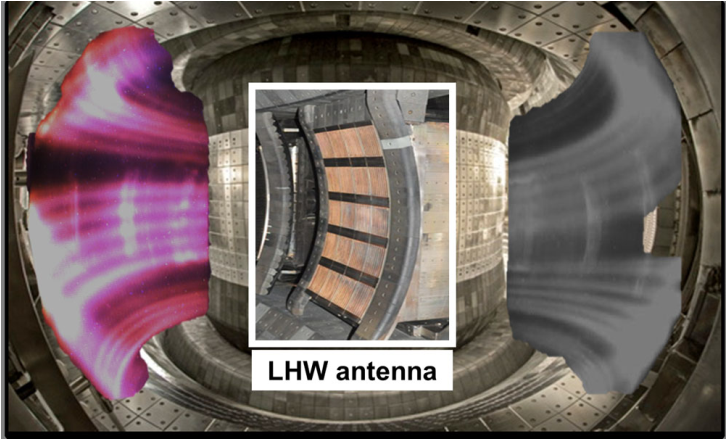
\includegraphics[width=0.70\columnwidth,keepaspectratio]{translate/liang_2.png}
  \caption*{图~2\hskip1em 图为 \east 环形腔内低杂波激发的螺旋辐射带,中间嵌入的图片为低杂波天线。}
  \label{fig:liang_figure2}
\end{figure}

\begin{figure}[h]
  \centering
  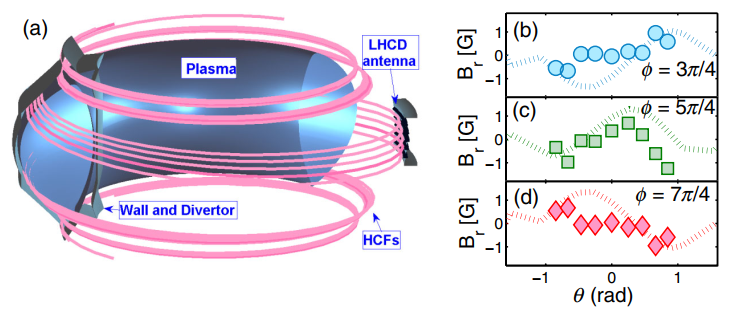
\includegraphics[width=0.85\columnwidth,keepaspectratio]{translate/liang_3.png}
  \caption*{图~3\hskip1em (a)螺旋电流丝模拟的示意图和测量到的低杂波产生的电流丝结构驱动的非轴对称的径向扰动场在不同的环向截面 $\phi=\text{const}$ 上的极向分布,(b)$\phi=2\pi/4$(c)$\phi=2\pi/4$(d)$\phi=2\pi/4$。极向角 $\theta$ 原点定义从低场侧赤道面,顺时针方向增加。环向角从低杂波天线所处的截面处为原点,从上往下看逆时针方向增加。模拟的螺旋电流丝总电流为 \SI{1.3}{\kilo\ampere} ,其对应计算得到的非轴对称的径向扰动场亦作图其中。}
  \label{fig:liang_figure3}
\end{figure}
% FIXME pitch angle

% FIXME Sentence ERROR, commented
在低杂波系统调制过程中,等离子体边界螺旋丝状结构中流动的电流(即螺旋电流丝,HCF,Helical Current Filament)所激发出来的磁扰动被 Mirnov 线圈观测到了。在这项实验中,低杂波被方波调制,功率周期性在 \SI{0}{\mega\watt}、\SI{1.2}{\mega\watt} 之间转换,重复频率是\SI{100}{\hertz},单周期内运转时长占 50\%。螺旋电流丝的产生是相当快速的,约\SI{2}{\milli\second}之内,和低杂波系统的启动时间相当。%低杂波系统开始工作时,下降沿的螺旋电流丝在几个毫秒之内便耗散了。
螺旋电流丝所引起的拓朴结构改变,在极向和环向上都是不对称的,这表明了它对等离子体结构的扭曲是三维的。用模拟的螺旋电流丝产生的扰动场可以复现 Mirnov 线圈上得到的信号,如图 3。其中螺旋电流丝被设定为螺旋辐射带中流过的电流,轨迹如图 3(a) 所示。总的螺旋电流丝电流可以通过拟合模拟的扰动场和测量值来计算,该实验中约为 \SI{1.3}{\kilo\ampere}。


\begin{figure}[h]
  \centering
  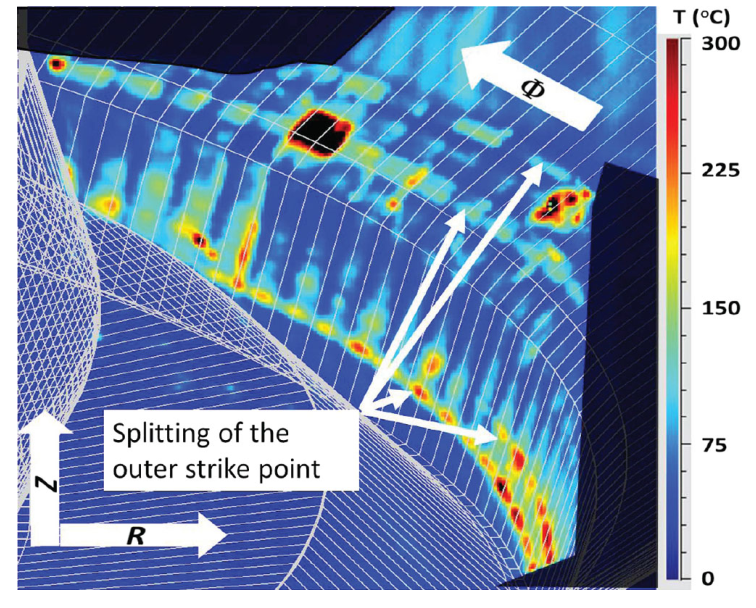
\includegraphics[width=0.65\columnwidth,keepaspectratio]{translate/liang_4.png}
  \caption*{图~4\hskip1em 低杂波工作时,腔外侧底部偏滤器的红外照片,环向角分布 $\phi=\SIrange{1.3\pi}{1.5\pi}{\rad}$}。在偏滤器平板上原打击点分裂为了多个条纹状结构。第一壁的结构由图中附加的网格白线所描绘。环向上打击点分裂的不对称性可由此见得。 
  \label{fig:liang_figure4}
\end{figure}

在低杂波系统运转的时候被观测到了在偏滤器上打击点(Strike points, SP)的分裂,这和共振磁扰动产生的影响相似,可以通过偏滤器平板上的热负荷分布上观察到,图 4 显示了红外摄像头测量到的外侧下部偏滤器平板的表面温度分布,可见原打击点发生了明显的多重分裂。打击点分裂前后在环向上的距离依赖于环向角,表明低杂波引起的磁扰动的三维特性。另外打击点分裂还取决于边界的安全系数,这一点在欧姆加热主导的和离子回旋加热主导的等离子体中都没有发现。

% FIXME Connection Length
% FIXME lobe modification


通过在磁力场线追踪的程序中考虑螺旋电流丝的扰动场影响,如图 5 ,本文定性地模拟了磁拓扑结构的改变。在实验平衡场基础上叠加螺旋电流丝(电流强度设为 \SI{1.3}{\kilo\ampere})产生的扰动场,通过磁力线追踪来计算磁力线的连接长度。螺旋电流丝产生的磁场在 X 点附近促进形成了数瓣有着较长磁连接长度的区域,甚至该区域可直达外侧偏滤器平板,导致打击点的分裂,这和红外摄像相互佐证。计算结果表明,等离子体边界的剧烈变化依赖于边界的安全系数和流经电流丝的电流强度。还要注意该螺旋电流丝模型没有考虑进去等离子体反馈,并且模拟的结果只能定性地解释螺旋电流丝引起的打击点分裂。



\begin{figure}[h]
  \centering
  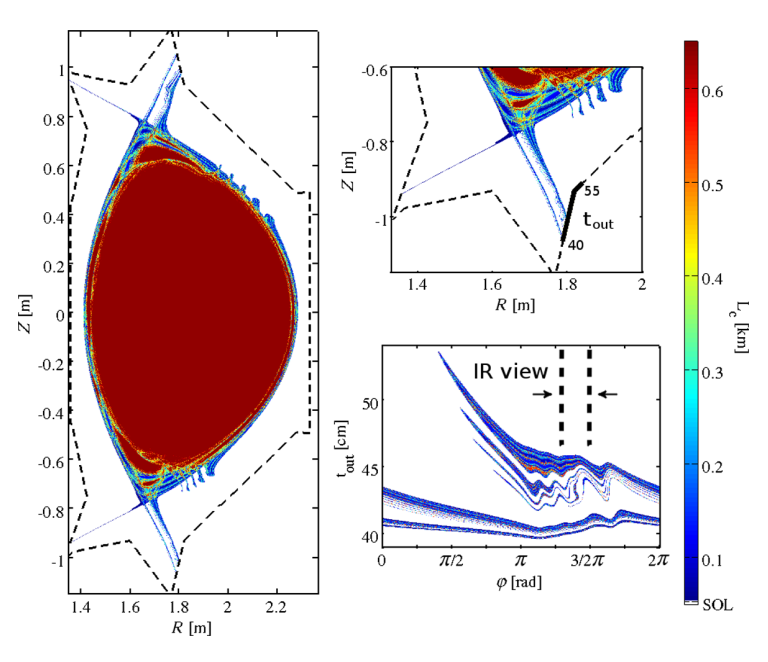
\includegraphics[width=0.85\columnwidth,keepaspectratio]{translate/liang_5.png}
  \caption*{图~5\hskip1em 完整极向切面上 $\phi=\SI{1.3\pi}{\rad}$ 的磁连接长度等值线图,底部偏滤器周围区域放大后如右上所示。在外侧偏滤器平板上磁力线落点和磁连接长度的对应关系如右下所示。计算依据于图 4 实验中重构的平衡场,其中红外摄像的范围作了标记。}
  \label{fig:liang_figure5}
\end{figure}



\begin{figure}[h]
  \centering
  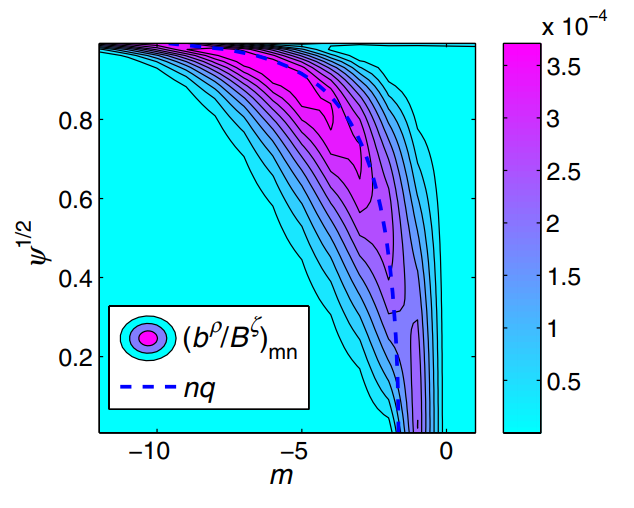
\includegraphics[width=0.65\columnwidth,keepaspectratio]{translate/liang_6.png}
  \caption*{图~6\hskip1em \SI{1}{\kilo\ampere} 螺旋电流丝产生的扰动场径向分量的磁谱 n=1,$m$ 表示极向模数,$\Psi$ 为归一化极向磁通。计算基于图 4 实验重建出的平衡场。其中螺旋共振模式 $m=nq(\Psi)$ 通过虚线做了标记。}
  \label{fig:liang_figure6}
\end{figure}

% FIXME small ELM
过去的的实验结果已经表明低杂波可以在 SN 偏滤器位型上(JET)产生带震荡型 ELM 的\Hmode 等离子体,也可以在限制器位型下产生没有 ELM 的\Hmode 等离子体(JT60)。然而,其具体的物理机制还未被充分研究。在 \east 上,对离子回旋共振加热占主导的较低密度等离子体($n_e/n^{GW}<0.5$,这里 $n^{GW}$ 为 Greenwald 密度极限),用恒定的低杂波功率可以得到一个 ELM 较平稳的\Hmode 等离子体,其有着混合的 \typeone 和小的 ELM。通过降低离子回旋共振加热对低杂波加热的比例,并提高等离子体密度,达到了一个稳定的持续发生小 ELM 的\Hmode 等离子体,并保持了 32 秒。低杂波激发的螺旋电流丝及其造成的磁拓扑改变的迹象合理地解释了为什么低杂波可以减弱或者抑制 ELM ,并且为何显著地改变了对偏滤器平板上的热负荷分布。对于这种现象背后物理机制的理解,需要考虑这种抑制效果与以下几个因素的依赖关系,(\textit{i}) 腔壁涂锂,(\textit{ii}) 等离子体台基区碰撞率,(\textit{iii}) 安全因子 $q_{95}$,它们将会在未来 \east 上的实验进行进一步的研究。

% Pitch resonant modes
由于低杂波天线几何因素的影响,由螺旋电流丝所驱动的共振磁扰动场主要是 $n=1$ 的分量,在这里 $n$ 指环向模数。基于实验参数计算出来的磁扰动场的谱表明螺旋电流丝的扰动场共振能力较好,如图 6 ,磁谱中值较高的分量形成的脊线与磁面螺旋对应的线相贴合。另外,螺旋电流丝所引起的磁扰动更多地位于等离子体边界,对核心部分没有显著的影响,这主要是由于螺旋电流丝在边界刮削层中沿着磁力线进行流动。因此,螺旋电流丝的迹线总是紧密地贴合着边界磁力线,而与边界安全系数无关。

还需要提到,尽管低杂波在刮削层中引起电流的现象已经被许多设备上观察到了,然而它的物理机制依然不清楚,在 \acmod 的实验装置上面,当我们将低杂波注入方向改变的时候,刮削层中的电流方向并不会发生改变。\acmod 上,在低杂波功率约 \SI{850}{\kilo\watt} 时,若等离子体运转在高密度工作区,在刮削层中估计电流强度可以高达约 \SI{20}{\kilo\ampere},而 \east 上低杂波功率为 \SI{1.3}{\mega\watt} 时,极向上积分得到的螺旋电流丝则约\SI{7}{\kilo\ampere}。
用 GENRAY-CQL3D 程序对考虑碰撞阻尼的二维刮削层模拟表明,对 \east 上运行的高密度等离子体而言,大概 10\% 的低杂波功率沉积在了刮削层中。实验观测到的结果表明刮削层中的电流过大以至于不能通过低杂波的碰撞吸收导致的电流驱动来解释。不过要注意,被刮削层吸收的低杂波功率会对偏滤器区域中性粒子的电离有所贡献,从而增强了从偏滤器平板两侧中较热较稀疏的一侧到较冷较稠密的一侧的沿着刮削层中的磁力线的热电流。

\east 过去的研究表明,随着低杂波功率或者等离子体密度的增长,螺旋电流丝电流强度均会增长。然而,螺旋电流丝所处的径向位置在等离子体边界附近刮削层中,而此处磁连接长度远远大于电子的平均自由程。为了用低杂波实现对 ELM 和偏滤器热负荷主动的控制,螺旋丝中电流强度对实验参数的依赖关系将会在 \east 上面更进一步地被研究。

总的来说,低杂波对于 ELM 强烈的影响已经在 \east 上面得到了呈现,它表明 ELM 在其作用下会消失,或者偶尔出现,它的频率会从 $\sim 150$ 增加到 $\sim\SI{600}{\hertz}$,当低杂波运转的时候,可通过驱动沿着刮削层磁力线且不随时间环向旋转的螺旋电流丝,来引起等离子体磁拓扑上显著的改变。这继而导致了在偏滤器上的打击点分裂,与共振磁扰动引起的效果相仿。在磁力线追踪程序中引入螺旋电流丝能较好地复现出来磁拓扑所观测到的改变。这为下一代的聚变反应堆(ITER 或 DEMO)提供了一种很有吸引力的手段来优化热负荷分布,并且同时能够抑制或者弱化 ELM 导致的极大的脉冲热负荷和粒子流强。

这项研究由中国国家磁约束聚变科学项目支持,项目序号为 No. 2013GB106003 和 No. 2011GB107001。在这里还要致谢德国亥姆霍兹协会的亥姆霍兹大学青年研究者团体  VH-NG-410。



\title{{\heiti \east 托卡马克上共振磁扰动对 ELM 的弱化效果到完全抑制的非线性转换过程}\\Nonlinear Transition from Mitigation to Suppression of the Edge Localized Mode with Resonant Magnetic Perturbations in the \east Tokamak[2]}

{\heiti 摘要:} {\kaishu 本文呈现了 \east 托卡马克上如何用共振磁扰动使得 ELM 从被减弱到抑制的非线性转换。这是第一次对射频加热占主导且转速较低的等离子体的 ELM 用共振磁扰动的方法进行抑制。在转化发生之后,边界磁拓扑的改变有两个迹象,线性磁流体动力学和真空的模拟结果等离子体反馈场渐变的相移和骤然的射向偏滤器的三维粒子束流。转换的阈值依赖于共振磁扰动场的磁谱、等离子体自身的旋转及扰动场的幅度。这表明非线性等离子体反馈引起的边界磁拓扑结构改变在用共振磁扰动的手段抑制 ELM 时很重要。}

% FIXME peeling like
无论是在实验室等离子体物理还是在空间等离子体物理研究中,磁场重联及其导致的拓扑变化在等离子体动力学中都扮演了一个重要角色。通过共振磁扰动所引起的边界随机场,被认为是抑制等离子体边界周期性破裂发生的一种可行手段;这种不稳定性也被称为 ELM ,起初在 \ddd 托卡马克中被观察到。 ELM 会对直面等离子体的材料形成瞬态热负荷,并下一代的聚变设备中(如 \iter)的实验中可能使得材料性能下降。等离子体边界压力梯度和电流中储存的自由能,由于边界磁场的随机化而减少,随机场将等离子体引入一个相对于 ELM 更稳定的状态。\ddd 上成功的实验,激励了其他托卡马克设备运用共振磁扰动以控制 ELM 。然而等离子体反馈场往往会屏蔽施加的共振磁扰动,并且可能显著降低磁场的随机性,这一机制能否成功应用还需研究。与拓扑结构改变不同,线性的拟剥离模磁流体力学反馈,已经被发现在 ELM 控制中扮演着很重要的角色。非线性的等离子体响应已于 JET 托卡马克中被观测到了。近期,\ddd 上发现了在 ELM 抑制阶段,施加 $n=2$ 共振磁扰动场而产生边界磁岛的可能形成机制。然而目前的研究有待进一步完善,ELM 被完全抑制和弱化之间的关键性区别仍不清楚,以及线性和非线性的等离子体反馈在 ELM 抑制上的作用仍有待研究。

这篇快报阐述了第一次对转速较低且射频加热主导的的等离子体,以低 $n$ 的共振磁扰动场驱动 ELM 抑制的效果,这可能对于未来聚变设备有着重要价值。这也是第一次 \east 工作在中等碰撞率状态时观测到 RMP 实现了完全的 ELM 抑制的效果,同时拓展了过去在 \ddd 和 KSTAR 的所做的抑制 ELM 的结果。目前发现,边界附近的磁岛和超过阈值的磁拓扑改变(考虑等离子体反馈的条件下),两者在 ELM 抑制中起着重要作用,这一发现也揭示了线性和非线性反馈在 ELM 抑制中起到的不同作用。

2014 年 \east 低场侧安装了两个阵列组成($2×8=16$)的一套灵活的腔内共轭场线圈系统。\east 团队通过 $n=1,2$ 的共振磁扰动,成功地实现了对转速较低且射频加热主导的的等离子体中 \typeone ELM 的减弱及完全抑制。


\begin{figure}[h]
  \centering
  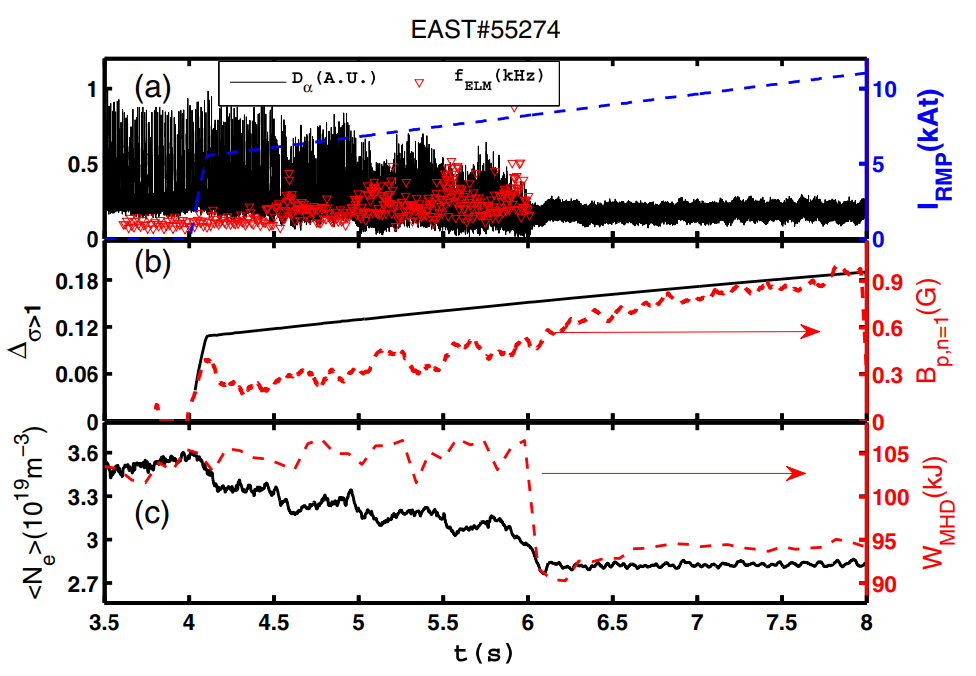
\includegraphics[width=0.85\columnwidth,keepaspectratio]{translate/sun_1.png}
  \caption*{图~1\hskip1em \east 55274 序号实验的各参数时间序列 (a) $D_\alpha$ (实线),ELM 频率(三角形)和 $I_{RMPs}$ (虚线)(b)$\Delta_{\sigma>1}$(实线)和 $n=1$ 反馈极向场幅度(虚线)(c)电子密度(实线)和等离子体储能(虚线)}
  \label{fig:sun_figure1}
\end{figure}


\east 中观测到,$n=1$ 的共振磁扰动场,强度超过阈值时具有对纯射频加热的等离子体 ELM 彻底抑制的效果。图 1 显示 \east 实验序号 55274 中,$n=1$ RMP 线圈电流缓慢上升过程中 ELM 的表现。低杂波电流驱动 $P_{LHCD}=\SI{3}{\mega\watt}$ 和离子回旋共振加热 $P_{ICRF}=\SI{1.4}{\mega\watt}$ 提供恒定的外部加热功率。 X 射线晶体成像技术(XCIS)测量得到等离子体环向上绕中心自旋的速度非常接近于0,(<\SI{4}{\kilo\rad\per\second})。环向磁感应强度为 $B_T = \SI{2.25}{\tesla}$,在边界 $95\%$ 的归一化极向磁通处的安全因子 $q_{95}\approx 5.7$,等离子体电流等于 $I_p=\SI{0.45}{\mega\ampere}$,归一化贝塔参数 $\beta_N \approx 0.8$,以及归一化的(相对于粒子轨道的碰撞或输运频率)碰撞率在基台顶部约等于 $\nu_{*e,ped}\sim 1$。如图 1 所示,RMP 线圈电流升到 \SI{8}{\kilo\ampere\cdot turns} 之前(\SI{6}{\second}),电子密度呈阶梯状下降并且 ELM 发生频率升高;而在 $t=\SI{6}{\second}$ 在此之后 ELM 被完全地抑制住了。
真空模拟中磁岛重叠处的宽度,如图 1(b) 黑实线,$\Delta_{\sigma>1}=1-\hat{\psi}_p^{1/2}|_{\sigma=1}$,此处 $\sigma$ 为 Chirikov 参数表征磁岛是否重叠而 $\hat{\psi}_p$ 指归一化之后的极向磁通。等离子体反馈在 ELM 的弱化和抑制两阶段起到的作用有着显著的不同。等离子体反馈场 $n=1$ 分量的幅度在实验中观测到的值可见图 1(b) 红实线。
在完全抑制之前,电子密度呈阶梯状的下降趋势而 ELM 频率有所增长,其原因可能是由于不同谐波分量有着不同的渗透阈值,说明(考虑等离子体反馈后的)磁拓扑结构改变的程度在最终的 ELM 抑制中非常重要。这激励团队对 ELM 在被弱化和抑制之间的转化过程进一步细致研究。



通过扫描托卡马克上下沿磁共振线圈的相位差 $\delta\phi_{UL}$,或者是等效的共轭分量场强,观察到了 ELM 减弱和抑制之间的转化。
图 2 展示了实验序号 55272 中操控 RMP 线圈对 ELM 的控制,连续扫描 $\delta\phi_{UL}$,如图 2(b)红线所示。通过以 $f=\SI{0.5}{\hertz}$ 的频率旋转下沿线圈电流,并且保持上沿线圈电流稳定,幅值恒定 $I_{RMP}= \SI{10}{\kilo\ampere\cdot turns}$,如图 2(a)中红虚线。该目标等离子体 ELM 的频率大致为 \SI{100}{\hertz} 与实验序号 55274 类似,除了加热手段上的略微不同,如有着 \SI{0.7}{\mega\watt} 的逆电流中性束注入而没有离子回旋共振加热。它仍然是射频加热主导的等离子体。$\delta\phi_{UL}$ 变化的两个阶段中,电子密度(图 2(c) 实线)和 ELM 频率(图 2(b) 三角形)的改变可重复性相当好,如图 4(a) 和 4(b) 。总的来说,$\delta\phi_{UL}$ 的变化可以分为两个阶段。在第一个阶段, $t\in[4,4.3 ]\text{s}\cup [6,6.3] \text{s}$ 对应于 $\delta\phi_{UL}\in [0,50]^\circ$, 此时有强烈粒子流溢出、 ELM 弱化以及 ELM 频率增大为原来的 5\~10 倍左右。阶段二 $t\in[4.3,4.7 ]\text{s}\cup [6.3,6.7] \text{s}$ 对应于 $\delta\phi_{UL}\in [50,120]^\circ$,在一个突兀的电子密度下滑之后 ELM 被完全地抑制住了。到 $\delta\phi_{UL}\in [120,360]^\circ$, ELM 从被完全抑制的第二阶段突然转化为第三阶段,等离子体密度溢出和弱化 ELM 的作用都变得相当弱且稳定了。电子密度和温度分布的变化在图 2(f)和 (g)中有所展示。从中可以看出在 RMP 的作用期间,电子密度下降但温度上升。等离子体能量约束在弱化 ELM 时相比没有启动 RMP 时有了些许的改善,储存能量更多但密度更低。与弱化 ELM 相比,完全地抑制 ELM 会有更强的密度泵出效应,且边界基台温度会轻微下降,从 ELM 的弱化到完全抑制,能量约束下降了大约10\%。

\begin{figure}[h]
  \centering
  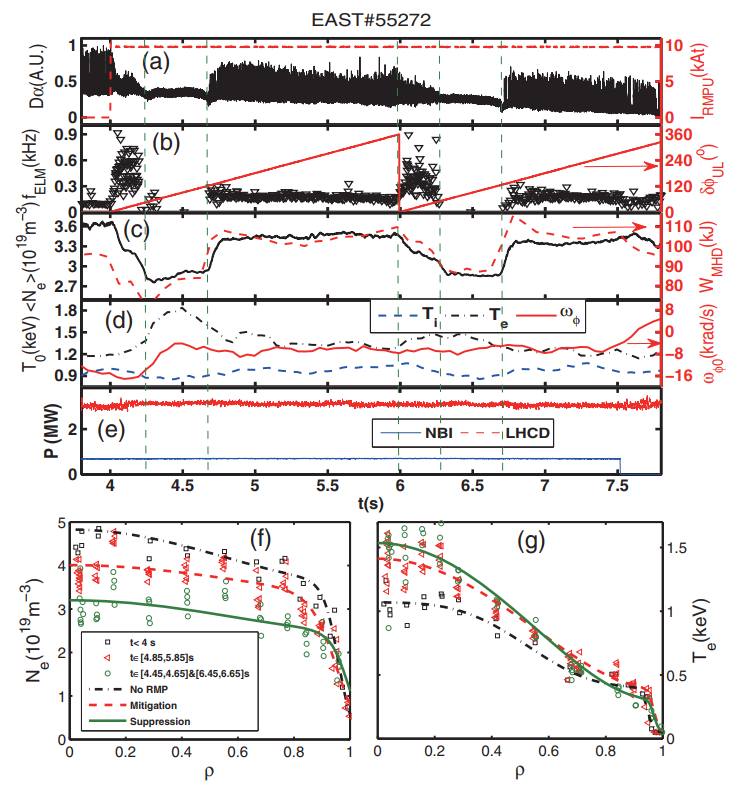
\includegraphics[width=0.85\columnwidth,keepaspectratio]{translate/sun_2.png}
  \caption*{图~2\hskip1em \east 实验序号 55272 一些参数的时间序列:(a)$D_\alpha$ 实线 和 RMPs 线圈电流 $I_{\text{RMPs}}$ 虚线;(b)ELM 频率(三角形)和 $\delta\phi_{\text{UL}}$ 实线;(c)电子密度为实线,等离子体储能为实线;(d)电子和离子的温度分别为点划线和虚线,近核心处环向旋转(实线);(e)NBI 功率为实线而 LHCD 功率为虚线。下面两子图为径向分布,(f)电子密度 和 (g)温度,点划线表示无 RMP 作用的时候,虚线和实线分别表示 RMP 起弱化和抑制作用的时候}
  \label{fig:sun_figure2}
\end{figure}

% FIXME ???? deepest poloidal flux
\begin{figure}[h]
  \centering
  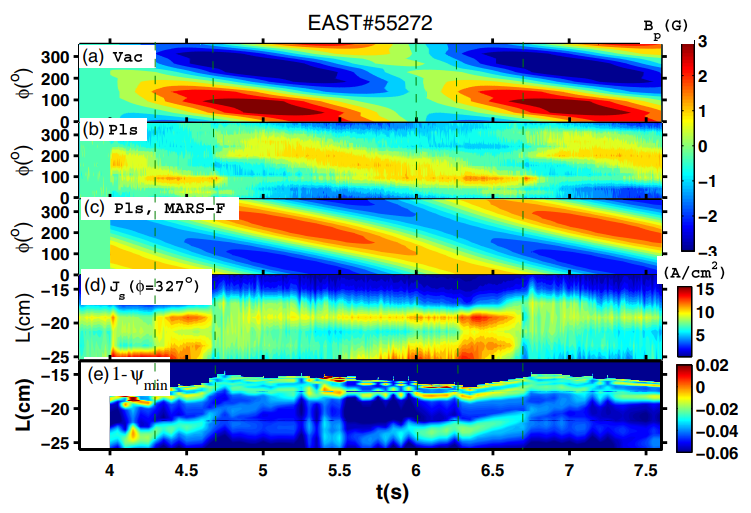
\includegraphics[width=0.85\columnwidth,keepaspectratio]{translate/sun_3.png}
  \caption*{图~3\hskip1em \east 实验序号为 55272 的扰动场时间演化的等值线图:(a)从 RMP 真空场中贡献的;(b)测量到的等离子体反馈;(c)\texttt{MARS-F} 模拟环向分布的磁传感器得到的等离子体反馈;(d)上沿偏滤器 $\phi=327^\circ$ 处的 Langmuir 探针极向阵列测量得到的粒子流强随时间的变化;(e)模拟的最深的连接上沿偏滤器的极向磁通}
  \label{fig:sun_figure3}
\end{figure}

\begin{figure}[h]
  \centering
  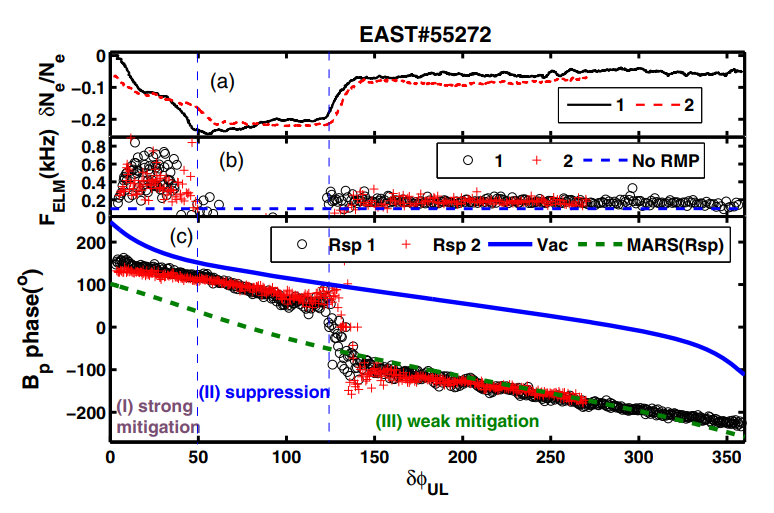
\includegraphics[width=0.85\columnwidth,keepaspectratio]{translate/sun_4.png}
  \caption*{图~4\hskip1em 一些变量受 $\delta\phi_{UL}$ 影响的散点和折线图:(a)等离子体密度;(b) ELM 频率;(c)测量得到的 $n=1$ 反馈场分量的相位(圆圈和加号分别表示第一阶段和第二阶段)及真空场模拟(实线)和线性 MHD 响应(虚线) }
  \label{fig:sun_figure4}
\end{figure}

 ELM 控制对磁谱的依赖性表明,共振磁扰动场需要达到必要的阈值才能抑制 ELM 。和在 \ddd 中观测到的类似, ELM 抑制最合适的相位差,和线性磁流体模拟程序 MARS-F 得到的共振峰值接近($\approx 75$ \degree),而与真空条件 MARS-F 计算出来的共振峰值计算($\approx 356$\degree)不吻合。然而,\east 上等离子体密度的时间演化和 \ddd 上完全不同,\ddd 上在 $\delta\Phi_{UL}$ 相位差扫描时等离子体密度抽出。并且磁刹车如同三角函数一个变化,显示出等离子体动理学特性的线性反馈。
% FIXME density pump-out and magnetic braking 
% TODO
实验测量结果清晰地表明 ELM 减弱和抑制之间的转换,存在着非线性等离子体反馈的作用以及非线性转换和分歧过程,如图 3 和 4 所示。\east 团队运用低场侧遍布环向各角度的极向磁场传感器(如图 3 所示)来观测等离子体反馈场的演化是。通过反馈场的傅立叶分解得出其主要的分量是 $n=1$ 的谐频分量。MARS-F 程序从等离子体反馈场中模拟出扰动场,在图 3(c) 中可以看出其较好地重现了总体的趋势,只有些许的不一样。实验序号 55272 在 $\SI{3.9}{\second}$ 的平衡态被用于这里展示的模拟,这是因为等离子体反馈场的预估,并不因有或者没有共振磁扰动导致的 ELM 抑制的磁场平衡态而产生显著的差异。
然而,$n=1$ 反馈场的相位对 $\delta\Phi_{UL}$ 的依赖关系(如图 4(c))明确地表征了 ELM 减弱和抑制之间的非线性特性。
弱 ELM 减弱阶段(III),$\delta\Phi_{UL}\in [120,360]$\degree, 测量到的 $n=1$ 反馈场和线性磁流体反馈相吻合,而在 ELM 抑制阶段(II)$\delta\Phi_{UL}\in [50,120]$\degree,它显著地偏离了线性的磁流体反馈却跟真空的更符合。
这表明共振磁扰动在 ELM 弱化状态被等离子体屏蔽掉了,到抑制状态却能够渗透进去。这是因为渗透的共振分量和真空中的一样有相同的相位;而根据过去的非线性模拟,屏蔽场相对于真空有一个相位偏移。这意味着为了达到 ELM 抑制状态,磁场渗透的发生是必需的,而这不能通过线性的模拟解释。这有可能解释 \ddd 中测量得到的反馈场和 MARS-F 模拟结果的类似的差异。
但和 \ddd 中观测到 ELM 抑制时的磁场渗透特性不一样的是,\east 上渗透的环向模数和施加的是一样的。


\begin{figure}[h]
  \centering
  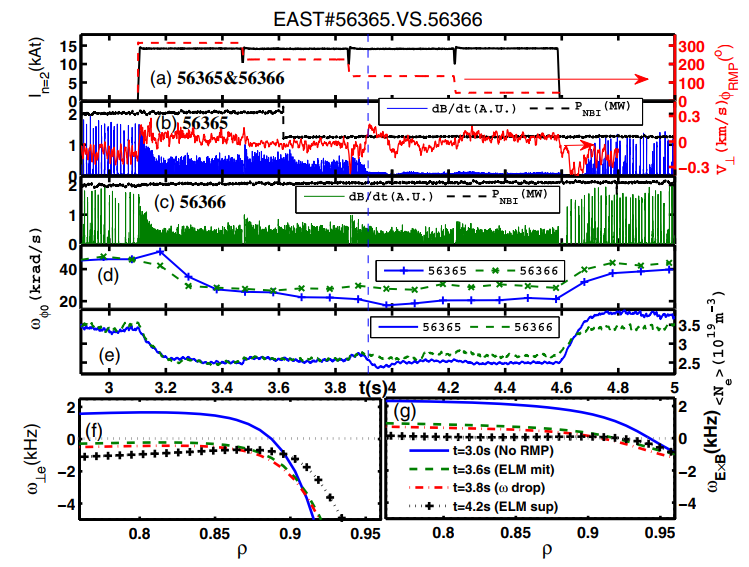
\includegraphics[width=0.85\columnwidth,keepaspectratio]{translate/sun_5.png}
  \caption*{图~5\hskip1em 一些参数的时间序列(a)幅度(实线)和相位(虚线)$n=2$ RMP 线圈电流, \east 实验序号 56365 和 56366(b)$dB/dt$ 实线,NBI 功率虚线和边界垂直转动为红线,\east 实验序号 56365 (c)$dB/dt$ 实线,NBI 功率虚线和边界垂直转动为红线,\east 实验序号 56366(d)在核心周围环向转动频率(e)电子密度。下面两小图为一些变量的径向分布,(f)$\omega_{e\perp}$ 和(g)$\omega_{E\times B}$ 在 $t=\SI{3.0}{\second},\SI{3.6}{\second},\SI{3.8}{\second}$ 和 $\SI{4.2}{\second}$  \east 实验序号 56365 }。
  \label{fig:sun_figure5}
\end{figure}

在 ELM 被减弱到完全抑制的转换过程中,反馈场的相位逐渐地和真空中的不断逼近,如图 4(c) 所示。这表明不同的谐频分量依次穿透,边界拓扑变化在这一阶段渐渐剧烈起来。对于不同的谐频分量来说渗透阈值可能是不一样的。于是一种可能的解释是这个转化过程中有多种谐频分量依次穿透。这也解释了在完全抑制 ELM 之前,共振磁扰动线圈电流的上升时,电子密度和 ELM 频率的阶梯状变化的现象,如图 1。于是,边界拓扑改变的剧烈程度随着总共振磁扰动场幅度增强而增强,这包括了等离子体反馈和它导致的 ELM 抑制。从抑制 ELM (阶段 \Romannum{2})到轻微减弱 ELM (阶段 \Romannum{3})的骤然反向转换表明这些共轭谐频分量又几乎同时被屏蔽掉了;同时,磁场的三维结构消失了,共振磁扰动场强度低于某个阈值之后。

% strong ELM mitigation ? 强的 ELM ? ELM 的强抑制?
在 ELM 抑制阶段,粒子流受共振磁扰动影响而在偏滤器上打击点的分裂,和边界拓扑结构的变化相互佐证。在 \ddd 上的\Lmode 等离子体,只有在等离子体屏蔽效应退去的时候,才能观测到三维的打击点分布。当共振磁扰动场强度超过阈值时,MAST 上\Lmode 等离子体出现粒子流和热负荷在偏滤器上的三维分布时,总是伴随着突然的热流增强和等离子体密度减弱,这表明存在边界随机场。
这已经在l模等离子体中被观测到了在max上面。这种分裂模式在强的 ELM 弱化阶段和抑制阶段,被观测到时用一个极向排列的兰缪探针阵列,在上偏滤器,在 $\Phi =327$\degree 的时候,观测到图 3,这和真空的三维模拟,打击点结果是相吻合的,显著的粒子流强增加,也表明了场的穿透和磁拓扑结构改变,在这些阶段,因为这是下 SN 位型,其中的两个分界面之间的距离 $d_{rsep}\approx \SI{1}{\centi\metre}$。这再一次证明了 ELM 抑制阶段存在边界磁拓扑的改变。
% 边界垂直转动 edge perpendicular rotation
从 ELM 弱化到完全抑制时,会突兀地加快边界垂直转动,再一次佐证 ELM 完全抑制时边界拓扑改变的重要性。外沿边界的加速旋转是边界随机场形成的重要迹象。图 5 显示了在两次实验 56365 和 56366 中,对 ELM 控制效果的对比,它们有着相同的共振磁扰动场参数为行,和目标等离子体,$B_T=\SI{1.7}{\tesla}$,$I_p=\SI{0.45}{\mega\ampere}$, $\beta\approx 1.5$ 和 $q_{95}\approx 4.5$。除了 56365 号顺向中性束功率为 \SI{2}{\mega\watt}在 $t\approx \SI{3.6}{\second}$ 降到 \SI{1.2}{\mega\watt},就如图 5(b) 所示。图 5(a) 一个阶梯,旋转共轭此共振磁扰动,有着这样子的类型,相位保持着恒定的电流 $I_{n=2}=\SI{14}{\kilo\ampere turns}$ 且 $\delta\Phi_{UL}=270$\degree,在这两次实验上都应用了。
这两次实验观测到了,共振磁扰动应用之后的 ELM 强烈减弱阶段,频率大概变为了原来的 5 倍。 ELM 的完全抑制,只有在一个额外的瞬间边界垂直旋转加速之后才会实现在一个缓慢的衰弱,由中性束功率的减低导致的等离子体旋转渐弱之后。 Mirnov 信号 $dB/dt$ 被用来作为测量 ELM 破裂的手段,因为它在 ELM 强削弱阶段对小 ELM 破裂更加敏感。如图 5(b) 所示,就在共振磁扰动施加之后,多普勒反散射系统观测到了边界垂直旋转的骤然加速,这表明边界拓扑结构的改变。而图 5(f),5(g) 展示了共振磁扰动启动后,因为旋转急停了,估计的电子流体垂直旋转角速度 $\omega_{e\perp}$,及$\vect{E}\times\vect{B}$ 对应的 $\omega_{E\times B}$ 在基座顶部俊变得非常接近于 0。根据近期的等离子体反馈理论和模拟结果,在基座顶部附近(此处 $\omega_{e\perp}\approx 0$)的共轭谐频分量可能渗透。在 ELM 抑制时,基座顶部处 $\omega_{e\perp}$ 又更接近于 0,此处 $\rho \approx 0.9$,而且$\omega_{E\times B}$ 在 $\rho=0.92$ 以内分布相当平坦。
更多的模式可能会渗透进等离子体,促成了最终的 ELM 抑制效果。以上论述表明强烈的 ELM 减弱效果和磁渗透及边界拓扑结构的改变是相关联的,并且最终到 ELM 完全抑制阶段的转换需要边界拓扑变化达到一定剧烈程度。

% pedestal top

在此总结, \east 托卡马克中观测到了,$n=1,2$ 的共振磁扰动驱动 ELM 弱化到完全抑制的非线性转化的迹象。实验中发现了对低速旋转、射频加热为主导的等离子体,低 $n$ 的共振磁扰动场有着抑制 ELM 的效果,这可能对于未来的聚变设备有潜在的重要价值。线性的磁流体模拟结果揭示了所需要的共振磁扰动场强度(需考虑等离子体反馈,而不仅仅是真空情况),从而可以据此优化设计适合抑制 ELM 的线圈位型,以完全抑制 ELM 。从 ELM 弱化到抑制的过程中,反馈场的相位逐渐地偏离线性磁流体模拟预测,而更接近于真空计算结果。
这表明不同的谐频分量依次渗透进等离子体,并且边界拓扑变化的程度在此过程中不断加深。这也解释了在达到 ELM 抑制之前,RMP 线圈电流不断抬升的过程中,观测到的电子密度和 ELM 频率阶梯状的变化。落入偏滤器的打击点分裂和粒子流强的突然增长说明 ELM 抑制阶段存在边界拓扑改变现象。另外,边界垂直旋转的急剧加速触发了从 ELM 弱化到抑制的转化,并且也表明存在着边界拓扑结构改变的阈值,到了便会完全抑制 ELM 。然而,模拟等离子体对共振磁扰动的非线性响应仍然是一个巨大的困难。未来更多的研究工作将会投入到理解非线性等离子体响应中,特别是对于其中转换和分歧的关键问题。

这项工作受到中国国家自然科学基金会的支持,项目序号为 No. 11475224 和 No. 11205199;同时还受到中国国家磁约束聚变科学计划支持,项目序号为 No. 2013 GB102000, No. 2013 GB106003B 和 No. 2012 GB105000.

% \chapter{其它附录}
% 前面两个附录主要是给本科生做例子。其它附录的内容可以放到这里,当然如果你愿意,可
% 以把这部分也放到独立的文件中,然后将其 \cs{input} 到主文件中。